\section{Estratégia de Busca}\label{sec:est_busca}

A estratégia de busca utilizada para gerar os novos estados a partir do estado
atual $x$ é apresentada na Figura~\ref{fig:estr_busca}.

\begin{figure}[H]
  \centering
  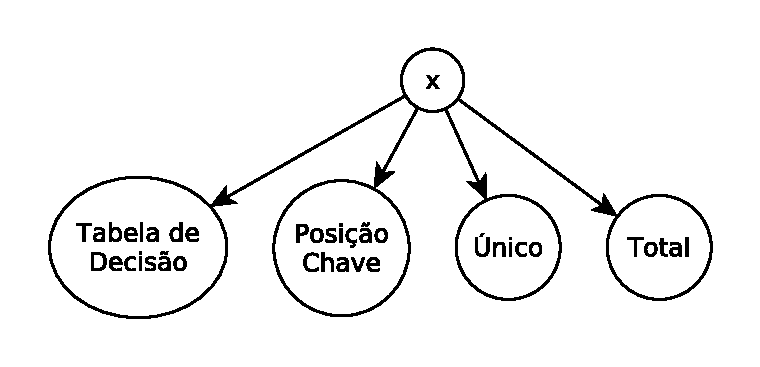
\includegraphics[width= 0.8\linewidth]{tab_dec}
  % TODO: mudar imagem
  \caption{Ilustração da distribuição dos estados
           considerados no planejamento}\label{fig:estr_busca}
\end{figure}

Os tipos de ações que são geradas são:
\begin{itemize}
  \item \textit{Tabela de decisão}: Ação escolhida no último planejamento;
  \item \textit{Único}: Ação gerada a partir da tabela de decisão onde a ação de
    um único robô foi modificada;
  \item \textit{Total}: Ação gerada a partir da tabela de decisão onde a ação do
    time completo foi modificada;
  \item \textit{Posição Chave}: Ação gerada utilizando posições chave (vide
    Seção~\ref{subsec:pos_chave}).
\end{itemize}

A ação selecionada é aquela que gera o maior valor de $f_U$.
O método da decida do gradiente foi implementado para melhorar
o planejamento. Calculando a série de Taylor para $f_U$ em torno
de $x_k$, tem-se:
\begin{dmath}
  f_U(x) = f_U(x_k) + \nabla f_U(x_k)^T(x-x_k) + O(\lVert x - x_k\rVert^2)
\end{dmath} 

Calculando no ponto $x_k + \gamma d$, com $\lVert d \rVert = 1$, tem-se:
\begin{dmath}
  f_U(x_k + \gamma d) = f_U(x_k) + \gamma \nabla f_U(x_k)^Td + O(\gamma^2)
\end{dmath} 

Para $\gamma$ suficientemente pequeno, tem-se que:
\begin{multline}
  f_U(x_k + \gamma d) - f_U(x_k) \approxeq \gamma \nabla f_U(x_k)^Td\\
  f_U(x_k + \gamma d) - f_U(x_k) > 0 \Rightarrow \gamma \nabla f_U(x_k)^Td > 0
\end{multline} 

Logo, tomando $d = \frac{\nabla f_U(x_k)}{\lVert \nabla f_U(x_k)\rVert}$ e
$\gamma > 0$, pode-se aumentar o valor de $f_U$ \cite{belegundu2011optimization}.

Como a taxa das soluções é fundamental para se controlar os robôs, pode-se
aplicar esse método de duas maneiras:
\begin{itemize}
  \item somente na melhor ação selecionada
  \item em todas as ações consideradas
\end{itemize}

A segunda opção reduz a taxa a zero pacotes por segundo, o que
prejudica o controle e invalida o planejamento, já que o estado
do jogo se modifica continuamente devido a ação do time adversário.

\subsection{Distribuição da Ação $Mover(r)$}\label{subsec:distr_mov}

Para gerar as ações do tipo $Mover(r)$, são utilizadas três distribuições
uniformes circulares. Essas distribuições tem centro na posição $r.pos$.
São utilizadas para concentrar localmente as movimentações de cada robô.

% vim: tw=80 et ts=2 sw=2 sts=2 ft=tex spelllang=pt_br,en

\subsection{Tabela de Decisão}\label{sec:tab_dec}
A tabela de decisão contém a memória das últimas
decisões $a_{old} \in A_c$ de todos os robôs de $T_c$.
Isso é incorporado ná próxima rodada do algorítmo,
conforme ilustrado na figura~\ref{fig:estr_busca}.


Devido a movimentação dos robôs em $Rob_{ad}$, somente as
ações $Mover(r_i)$ e $Chutar(r_{com{\ }bola})$ são guardadas
intergralmente. No caso da ação $Passar(r_j, r_{com{\ }bola})$,
devido a restrição de o robô que recebe interceptar a bola
antes dos robôs em $Rob_{ad}$, o calculo do receptor $r_j$ é
feito a cada rodada. O receptor anterior só entra no custo
da mudança (vide secção~\ref{subsec:change_cost}). 

Caso a posse de pola passe para o time adversário, o robô
que possuia a bola anteriormente fica com a sua última
ação do tipo $Mover(r_i)$.

\section{Posições Chave}
% TODO
em produção


% vim: tw=80 et ts=2 sw=2 sts=2 ft=tex spelllang=pt_br,en
